\chapter{Spectra and graphics}
% \ifpdf
% \begin{SCfigure}[H]
%  \centering
%  \subfigure[UV-vis spectrum of phosphite ligand \cmpd{legante}.\label{sp:uvvis-legante}]{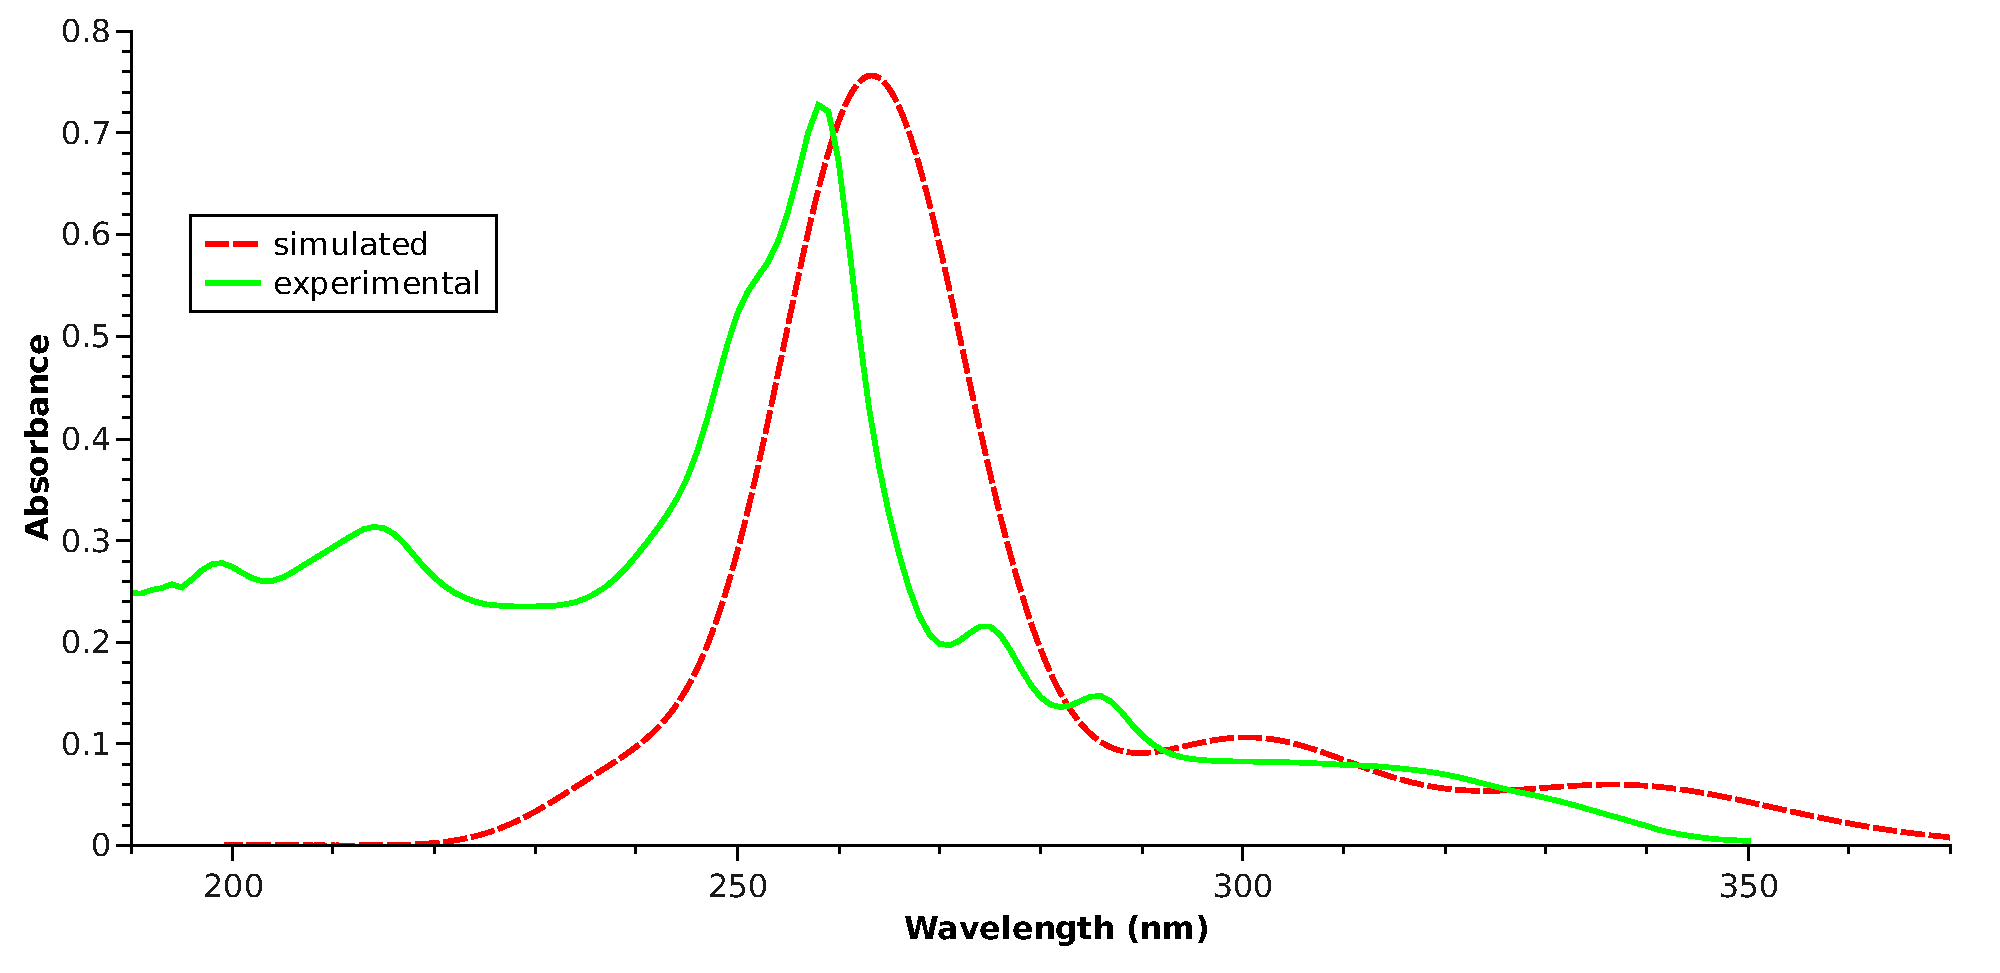
\includegraphics[width=0.5\textwidth]{sp/uvvis-sper-calc.pdf}}
%  \subfigure[Circular dichroism spectrum of phosphite ligand \cmpd{legante}.\label{sp:cd-legante}]{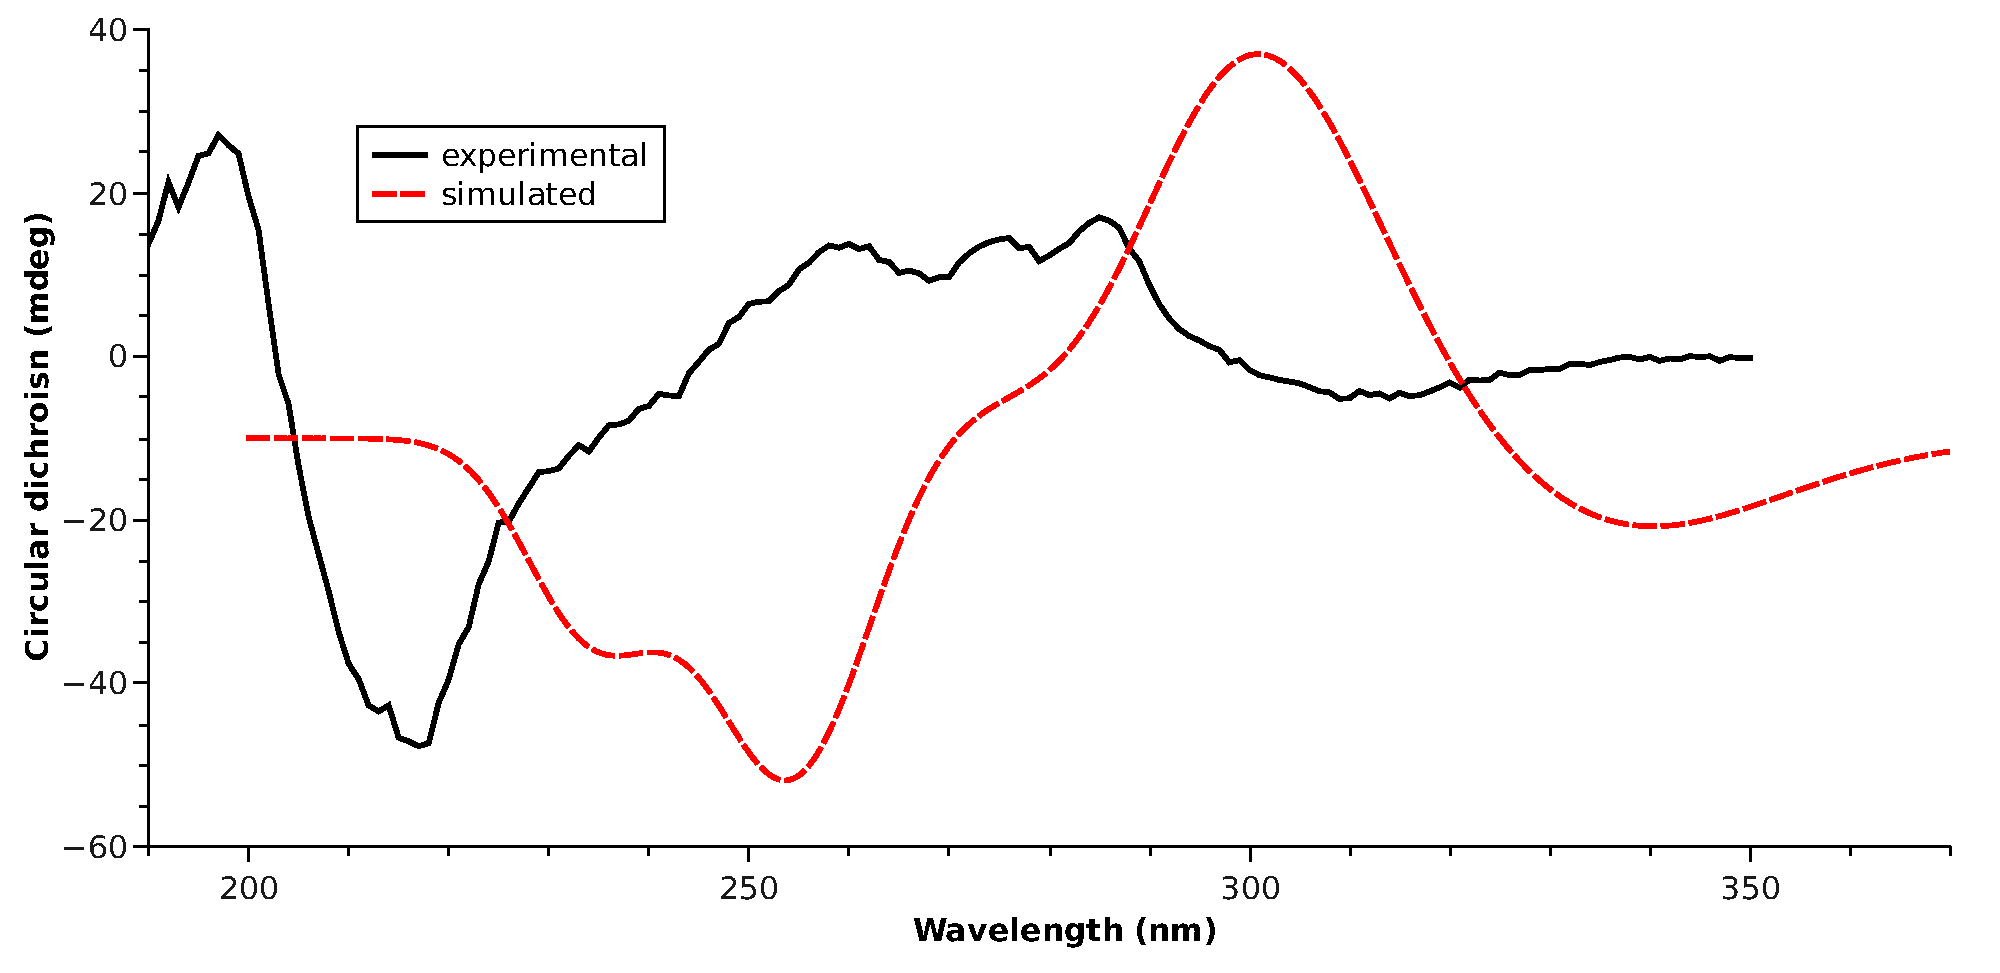
\includegraphics[width=0.5\textwidth]{sp/cd-sper-calc.pdf}}
% \caption{\\Experimental and calculated UV-vis and CD spectra of our ligand \cmpd+{legante}.}
% \end{SCfigure}
% \else
% \fignoeps
% \fi





\ifpdf
\begin{SCfigure}%[H]
 \centering
 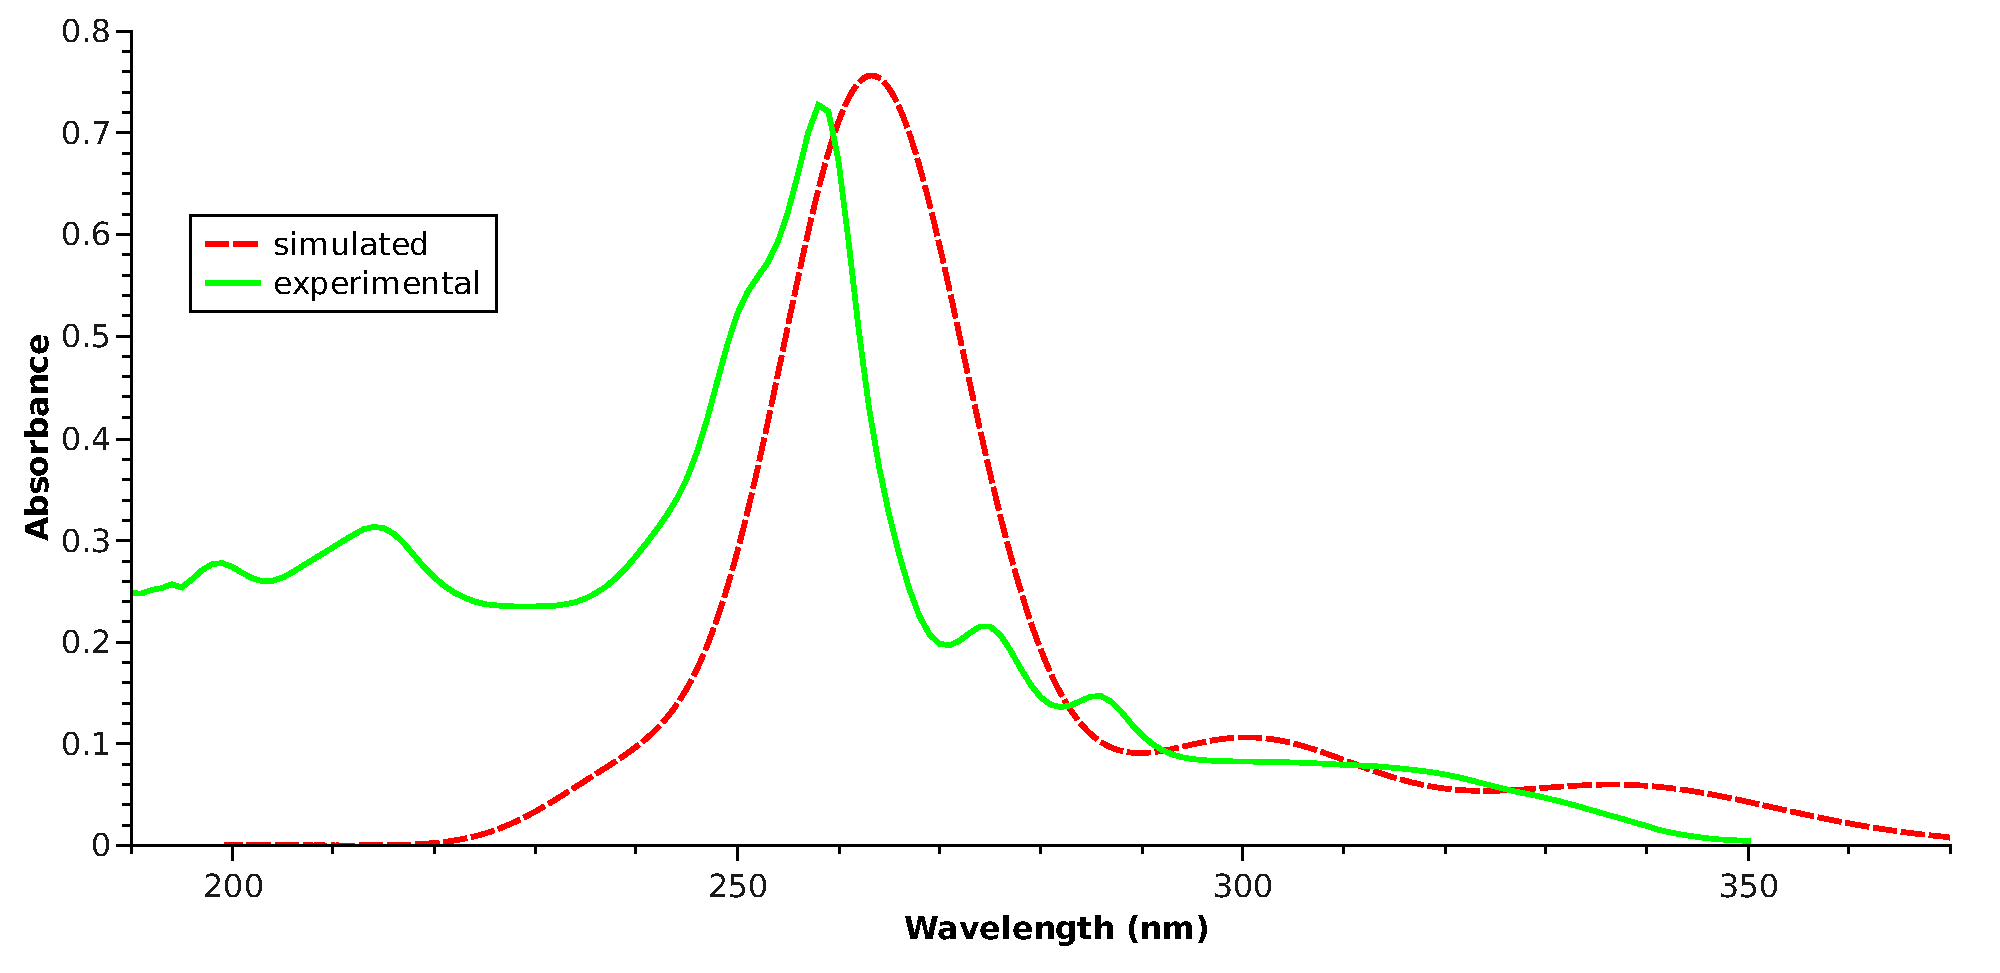
\includegraphics[width=1\textwidth]{sp/uvvis-sper-calc.pdf}
  \caption{\\Experimental and calculated UV-vis spectrum of phosphite ligand \cmpd{legante}.\label{sp:uvvis-legante}}
\end{SCfigure}
\begin{SCfigure}%[H]
 \centering
 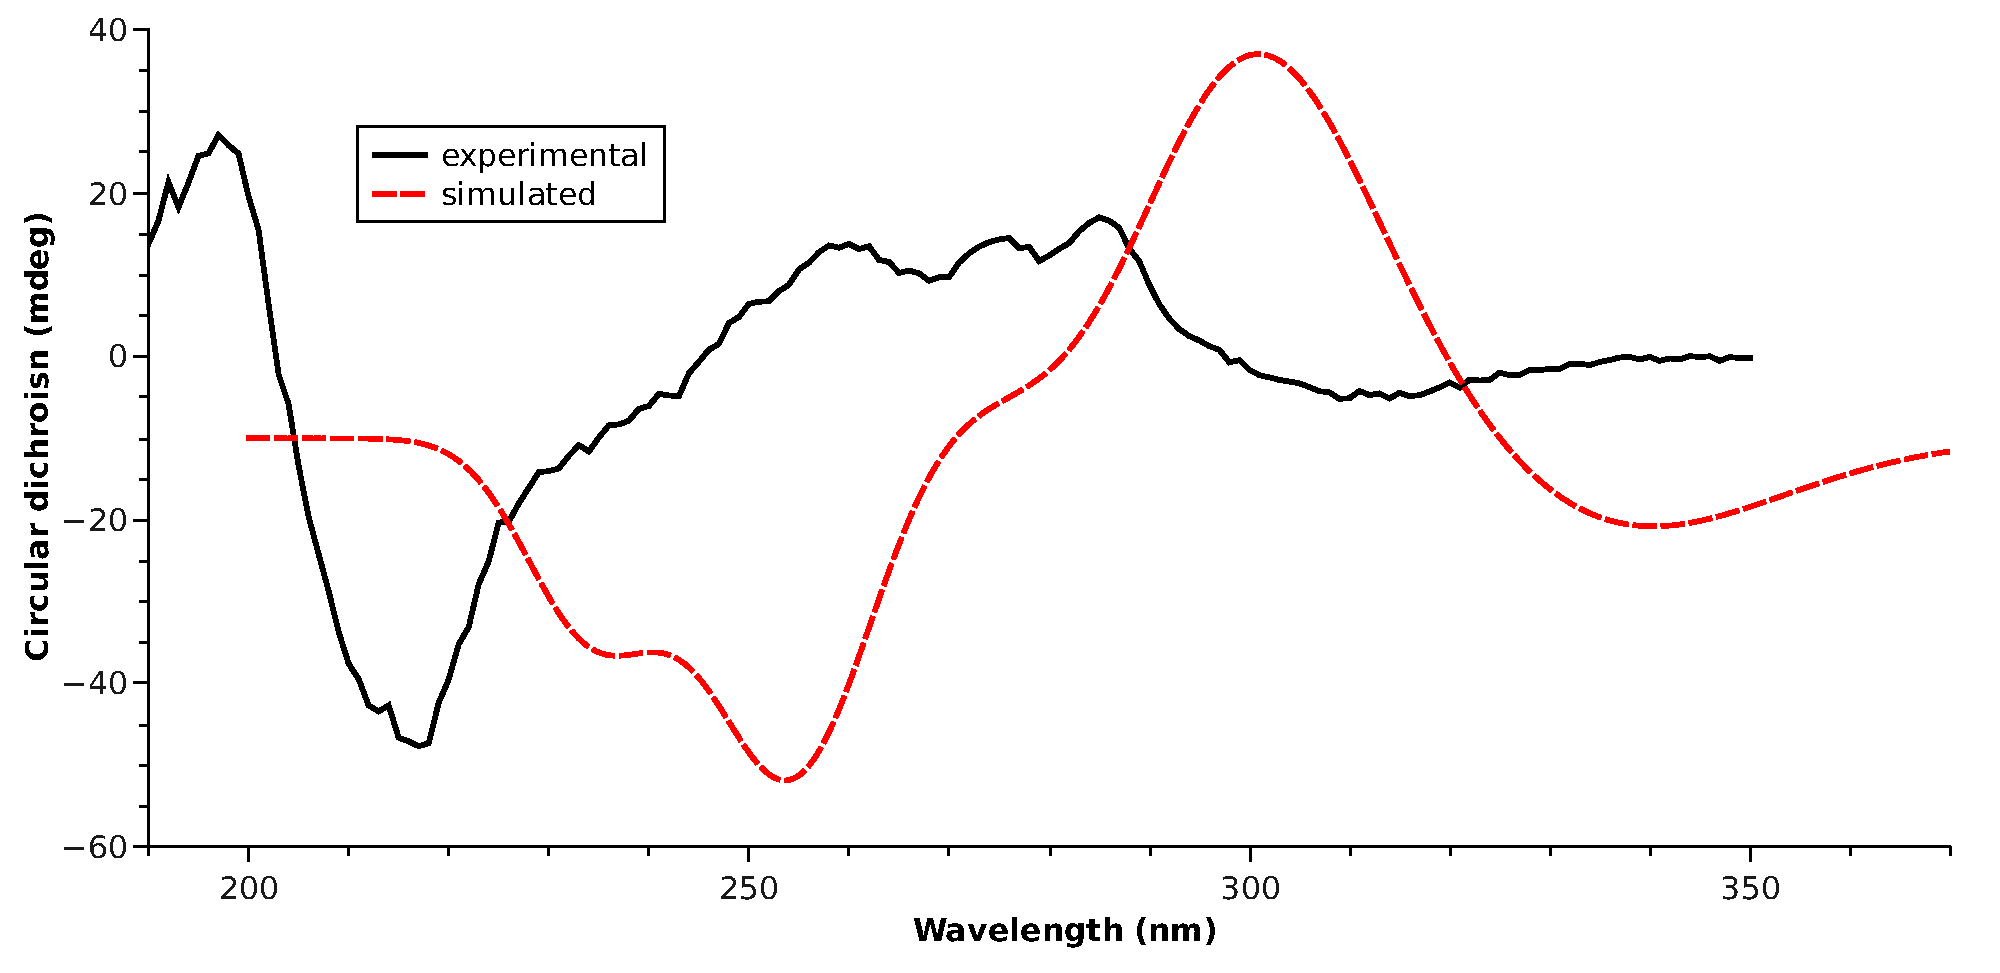
\includegraphics[width=1\textwidth]{sp/cd-sper-calc.pdf}
  \caption{\\Experimental and calculated circular dichroism spectrum of phosphite ligand \cmpd{legante}.\label{sp:cd-legante}}
\end{SCfigure}
\else
\fignoeps
\fi





\ifpdf
\begin{SCfigure}
  \subfigure[LUMO.\label{sp:lumo}]{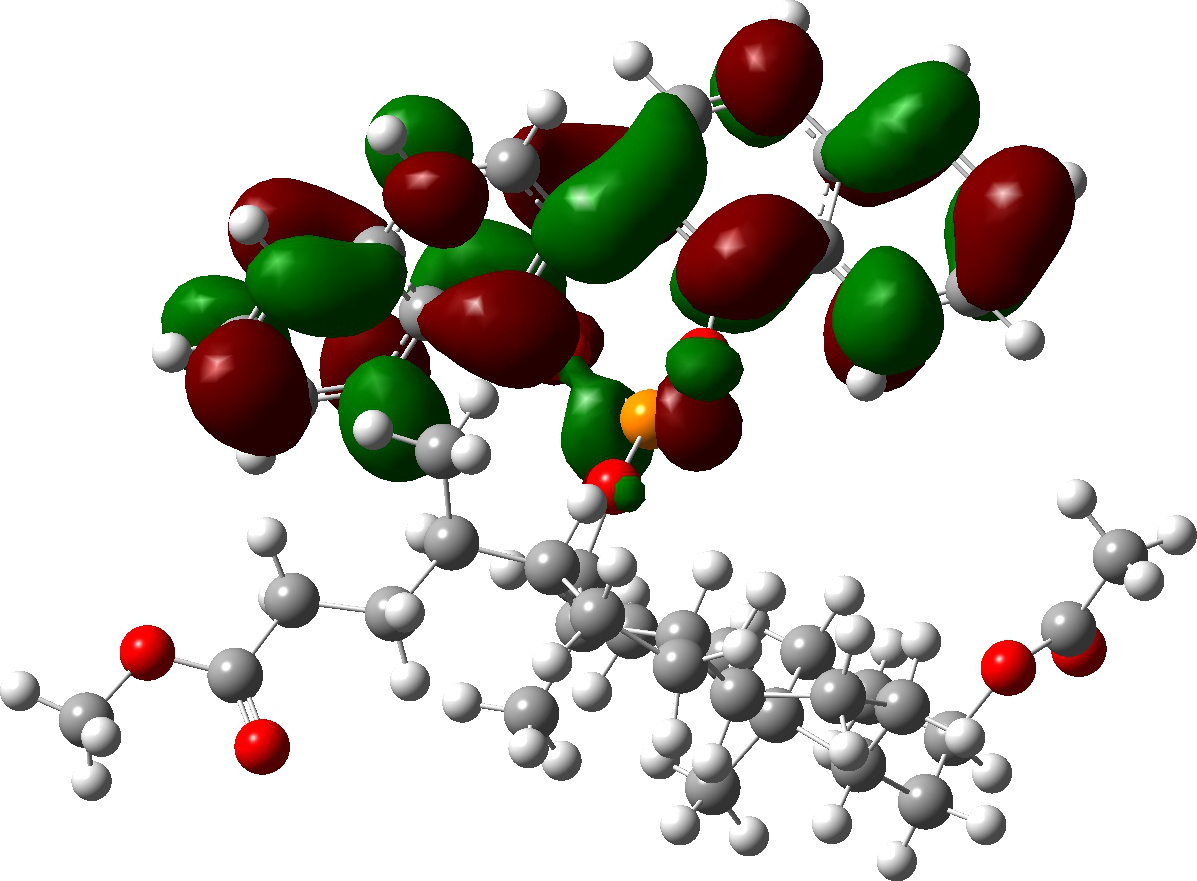
\includegraphics[width=0.87\textwidth]{sp/lumo-hq-crop.jpg}}
  \vspace{20pt}
  \subfigure[HOMO.\label{sp:homo}]{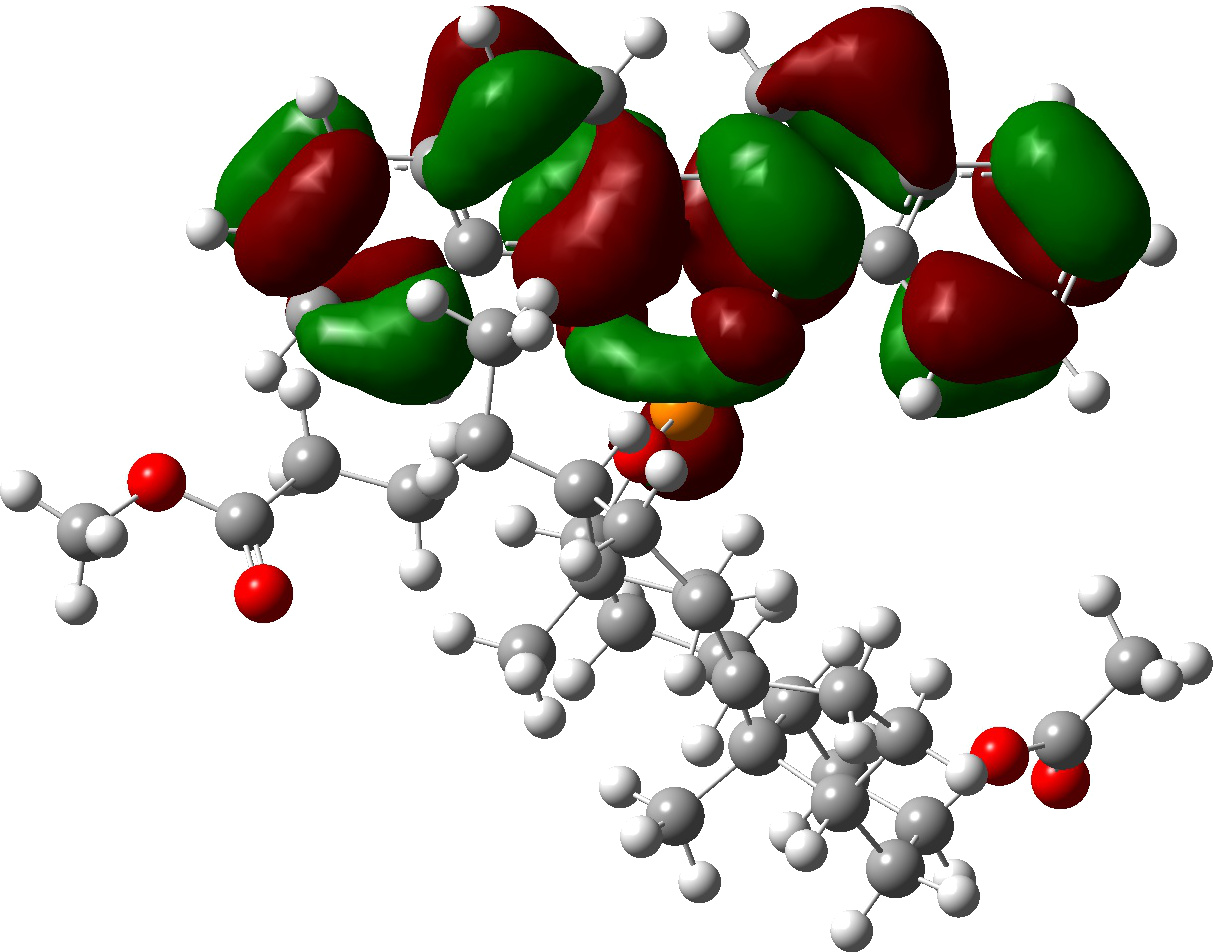
\includegraphics[width=0.87\textwidth]{sp/homo-hq-crop.jpg}}
\caption{\\Calculated LUMO and HOMO electronic levels of our ligand \cmpd+{legante}.}
\end{SCfigure}
% \begin{SCfigure}
%  \centering
%  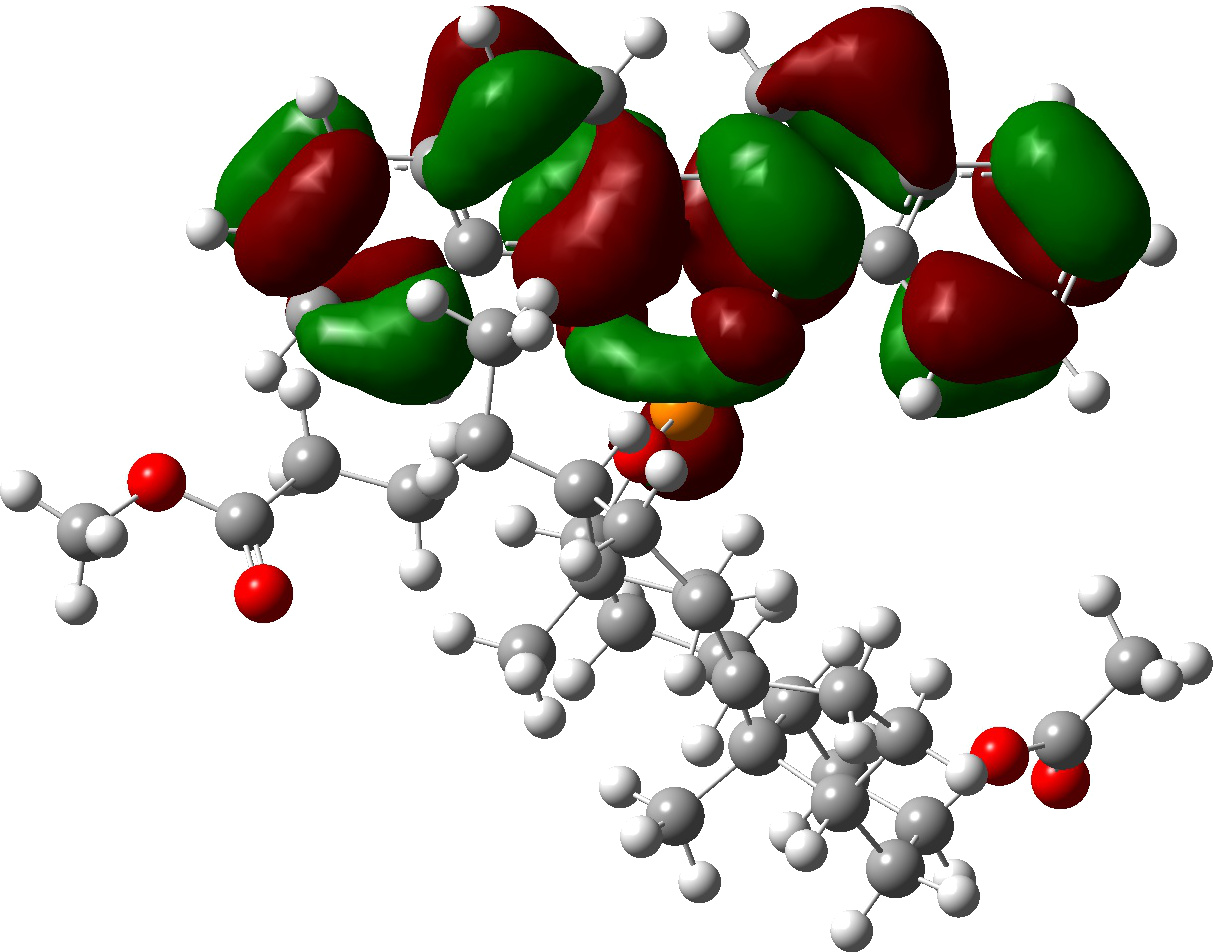
\includegraphics[width=1\textwidth]{sp/homo-hq-crop.jpg}
%  \caption{\\Calculated HOMO of our ligand \cmpd+{legante}.\label{sp:homo}}
% \end{SCfigure}
% \begin{SCfigure}
%  \centering
%  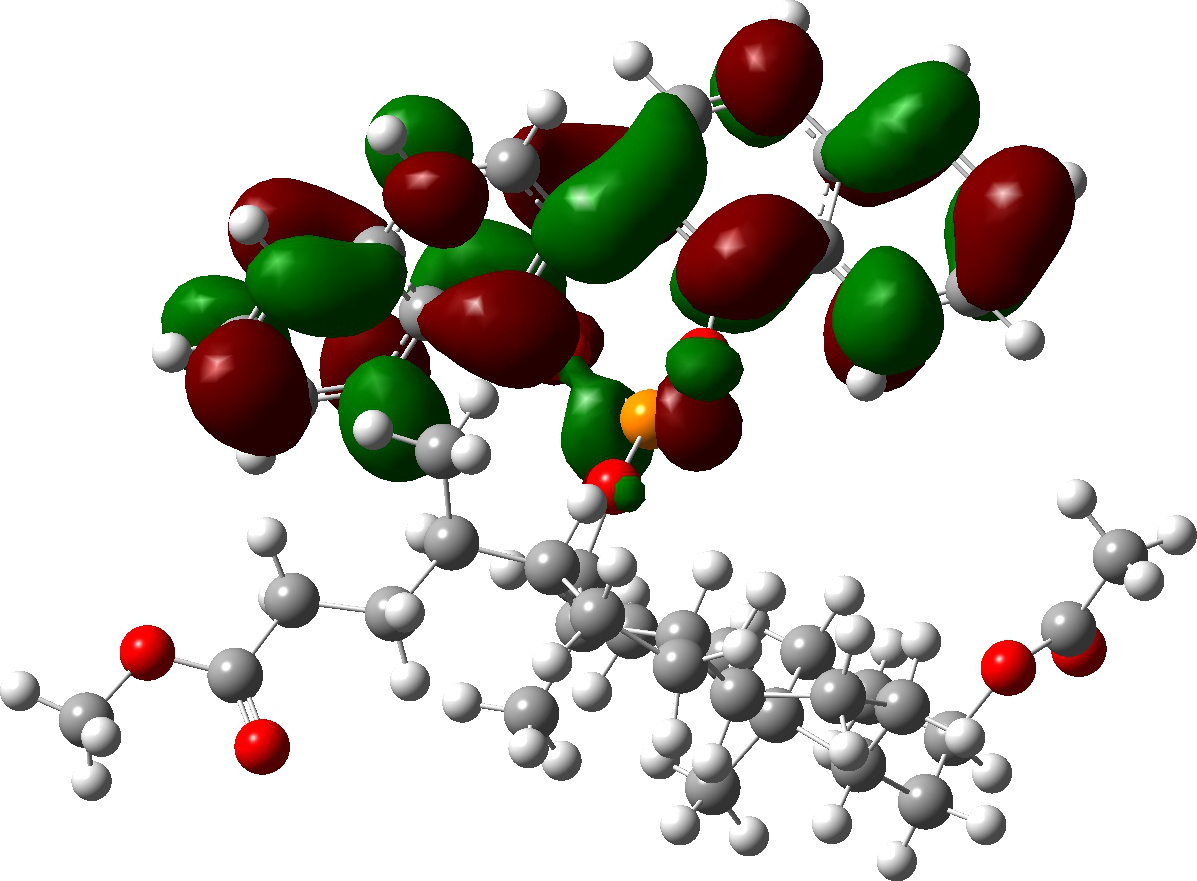
\includegraphics[width=1\textwidth]{sp/lumo-hq-crop.jpg}
%  \caption{\\Calculated LUMO of our ligand \cmpd+{legante}.\label{sp:lumo}}
% \end{SCfigure}

\else
\fignoeps
\fi


\ifpdf
\begin{SCfigure}%[H]
 \centering
 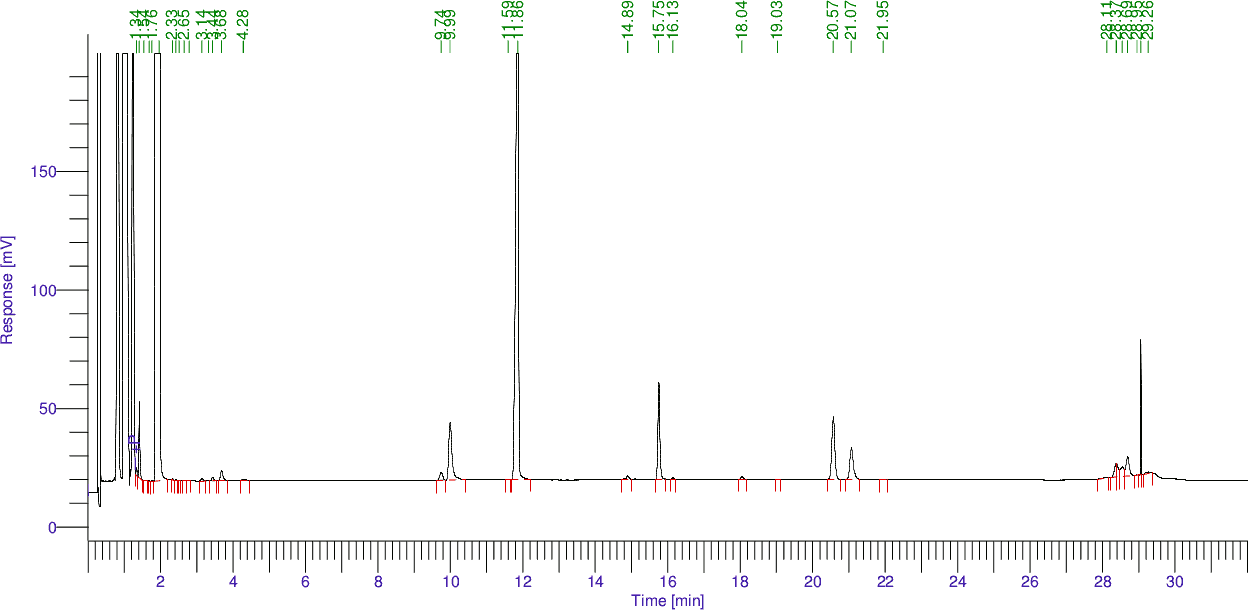
\includegraphics[width=1\textwidth]{sp/gc-indicizzato16.png}
  \caption{\\GC-FID analysis of the reaction mixture from conjugate addition.\label{sp:gc}}
\end{SCfigure}
\begin{SCfigure}%[H]
 \centering
 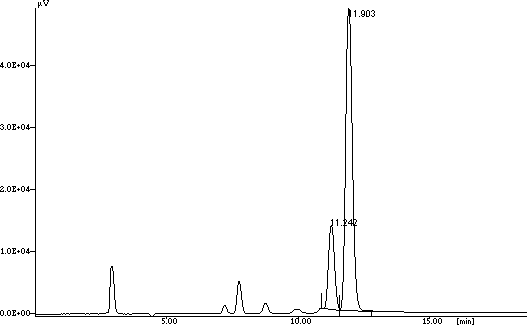
\includegraphics[width=1\textwidth]{sp/hplc.png}
  \caption{\\Chiral HPLC (Lux\textsuperscript{\textregistered} Cellulose-1), \n-hexane:isopropyl alcohol 95:5, flux 1~mL/min, column heated \SI{60}{\celsius}, wavelength 220~nm.\label{sp:hplc}}
\end{SCfigure}
\else
\fignoeps
\fi




\ifpdf
\begin{SCfigure}%[h]
 \centering
 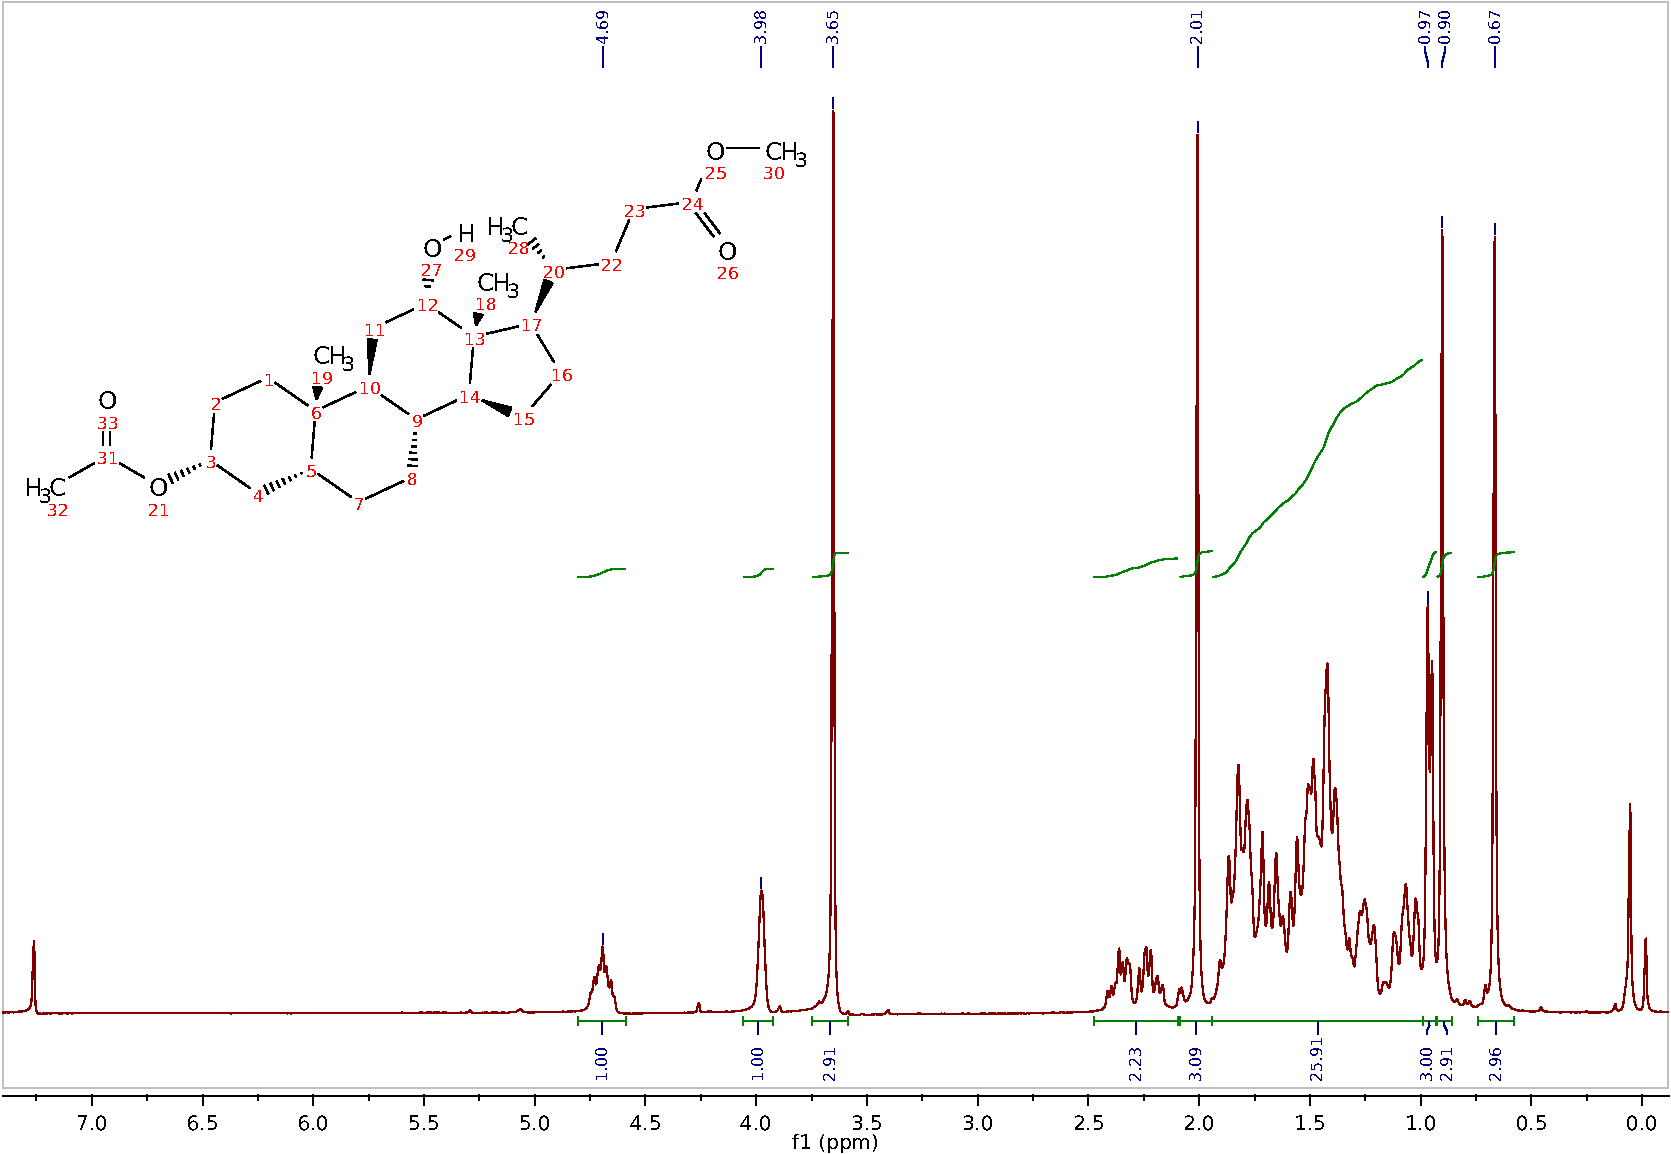
\includegraphics[width=1\textwidth]{sp/amda-crop.pdf}
  \caption{\\$^1$H-NMR (300~MHz, \ce{CDCl3}) spectrum of 3$\alpha$-acetyloxy-12$\alpha$-
hydroxy-7-deoxy\-cholic acid methyl ester \cmpd{amda}. \label{sp:amda}}
\end{SCfigure}
\else
\fignoeps
\fi

\ifpdf
\begin{SCfigure}%[h]
 \centering
 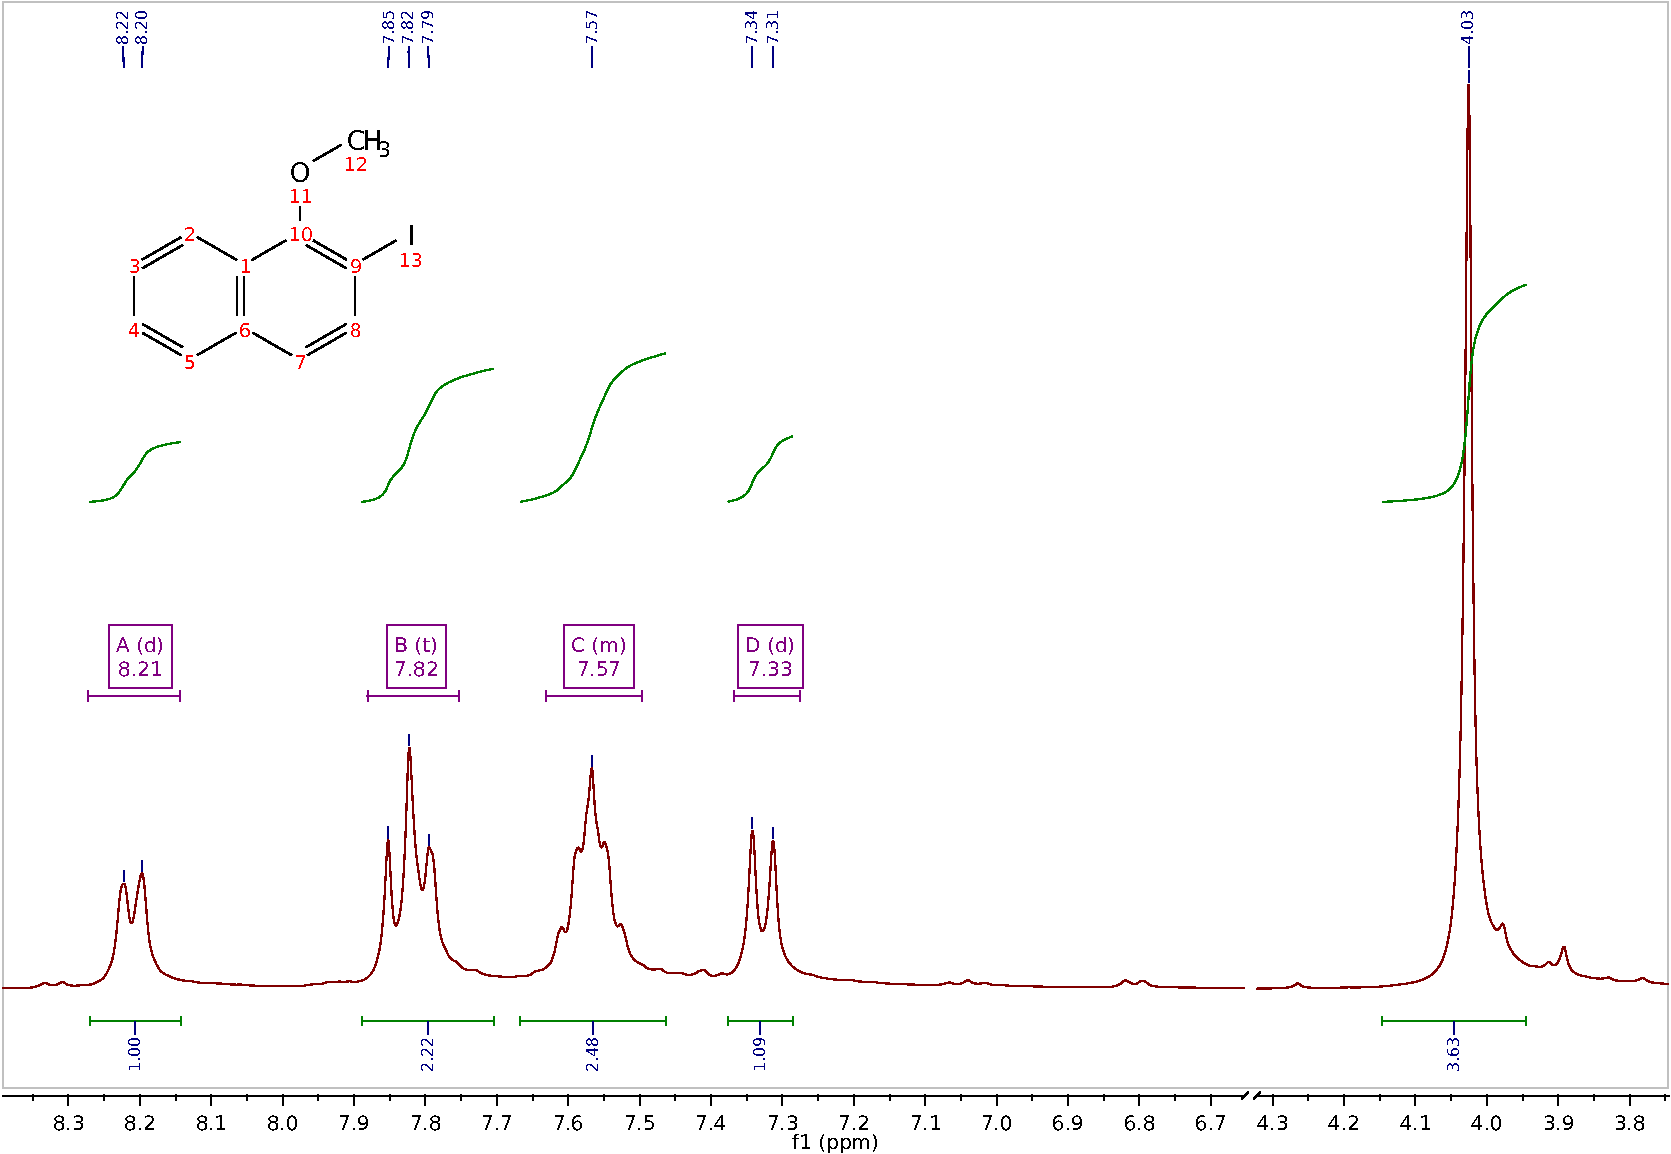
\includegraphics[width=1\textwidth]{sp/moni-crop.pdf}
  \caption{\\$^1$H-NMR (300~MHz, \ce{CDCl3}) spectrum of 2-iodo-1-methoxy\-naphthalene \cmpd{moni}. \label{sp:moni}}
\end{SCfigure}
\else
\fignoeps
\fi


\ifpdf
\begin{SCfigure}%[h]
 \centering
 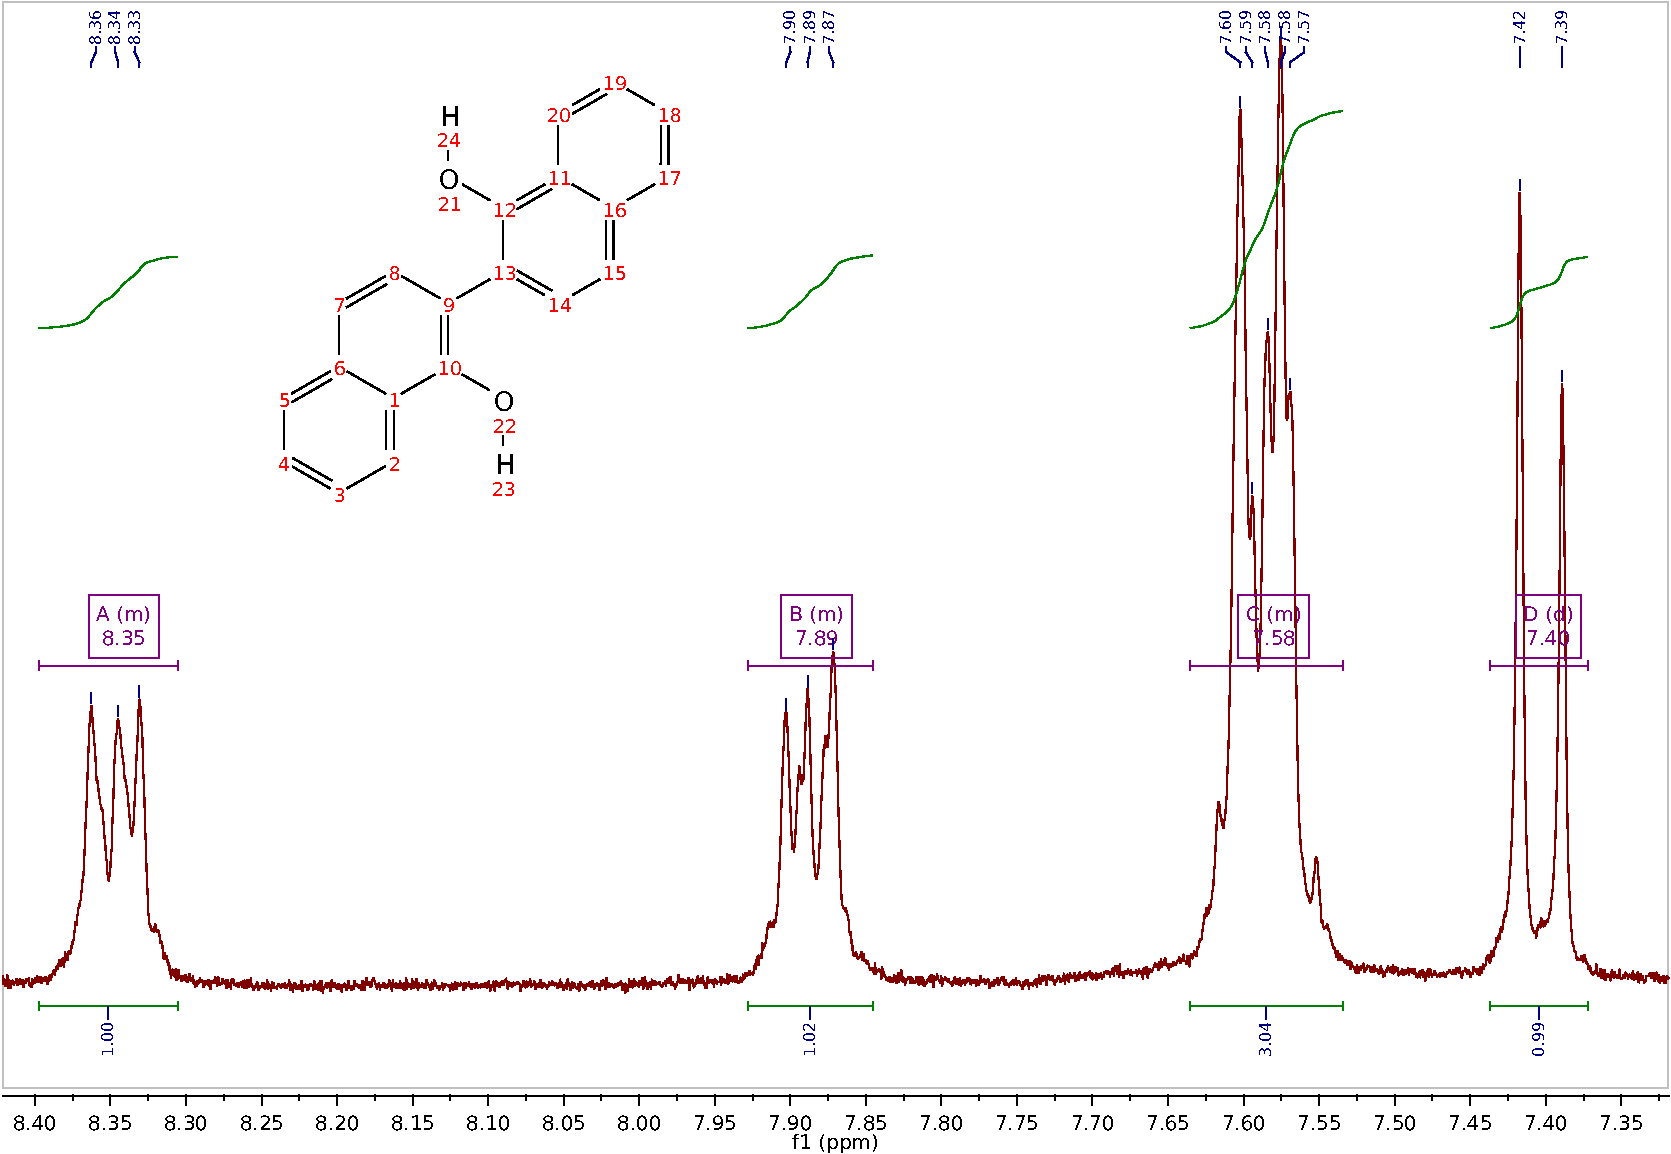
\includegraphics[width=1\textwidth]{sp/dhn-crop.pdf}
  \caption{\\$^1$H-NMR (300~MHz, \ce{CDCl3}) spectrum of 1,1'-dihydroxy-2,2'-binaphthalene \cmpd{dhn}. \label{sp:dhn}}
\end{SCfigure}
\else
\fignoeps
\fi


\ifpdf
\begin{SCfigure}%[h]
 \centering
 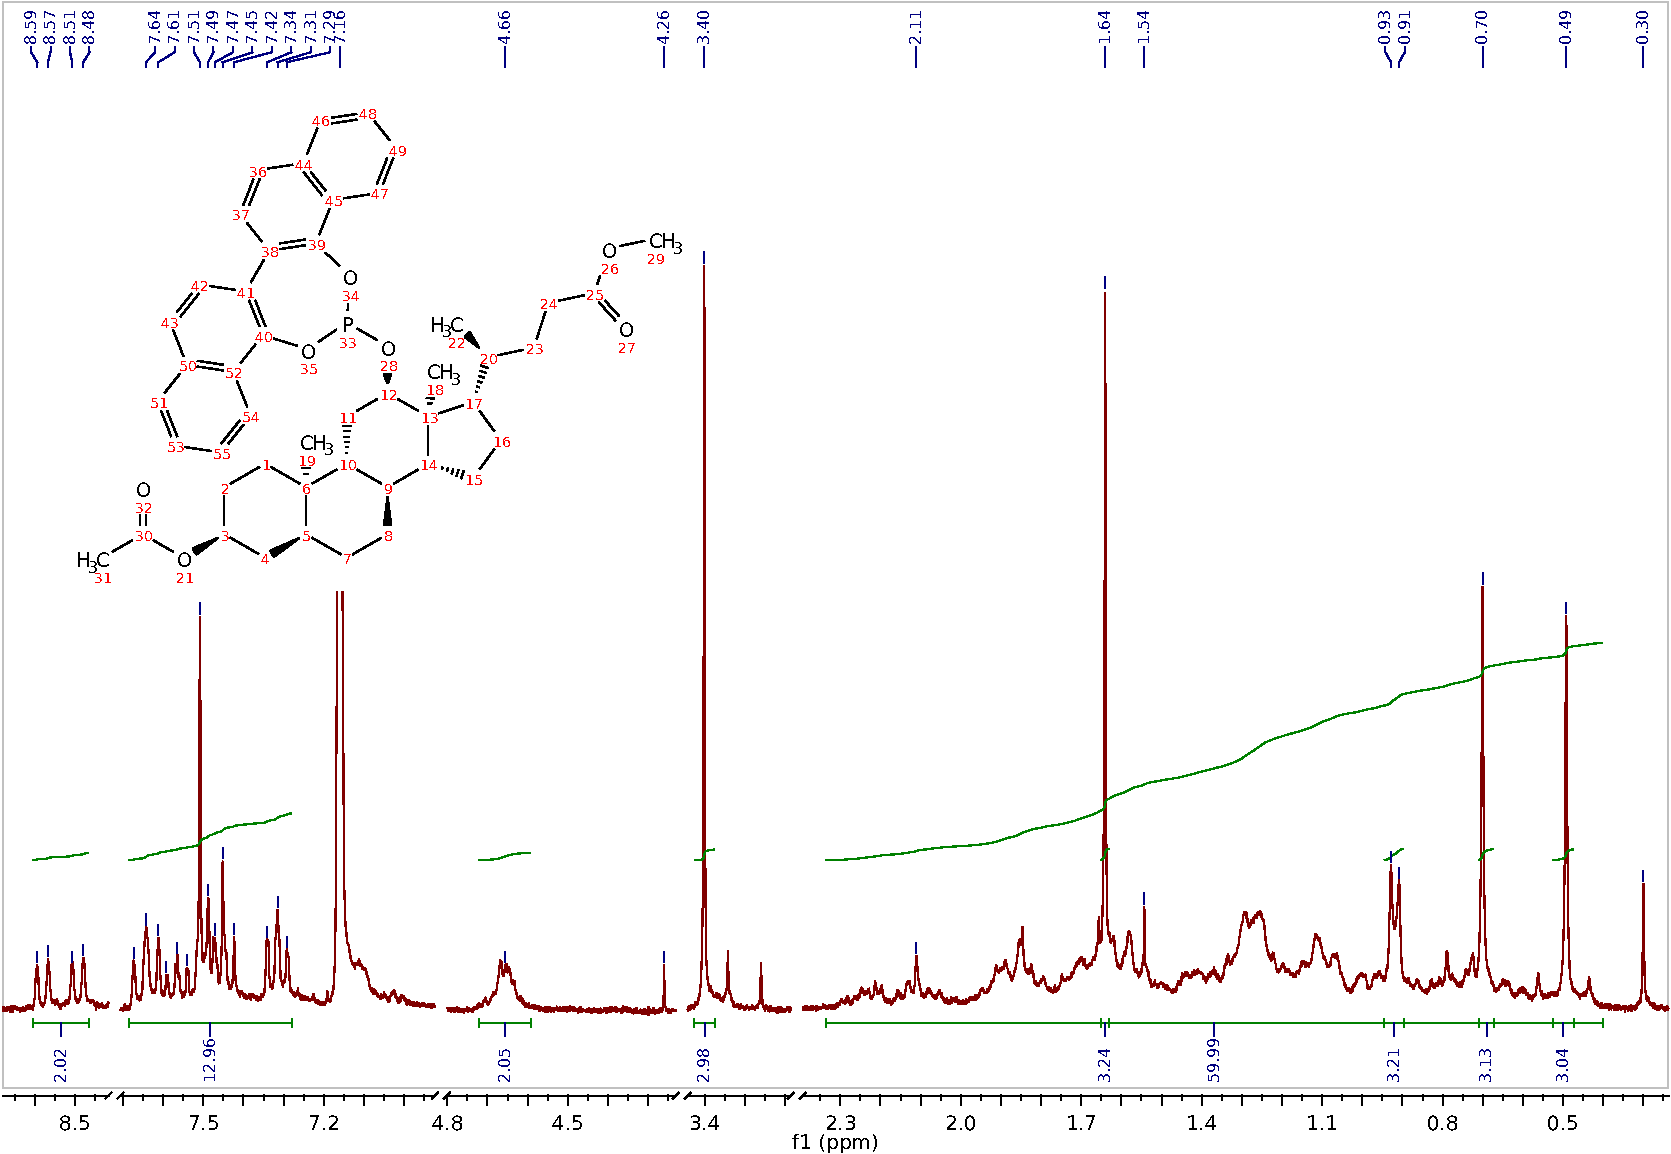
\includegraphics[width=1\textwidth]{sp/legante-crop.pdf}
  \caption{\\$^1$H-NMR (300~MHz, benzene-d6) spectrum of phosphite ligand \cmpd{legante}. Identified impurities: $\delta$ 7.16 (\ce{C6D5H}), 4.26 (\ce{CH2Cl2}), 2.11 (toluene), 1.54 (acetone), 0.30 (maybe water). \label{sp:legante}}
\end{SCfigure}
\else
\fignoeps
\fi

\begin{landscape}

\ifpdf
\begin{figure}%[h]
 \centering
 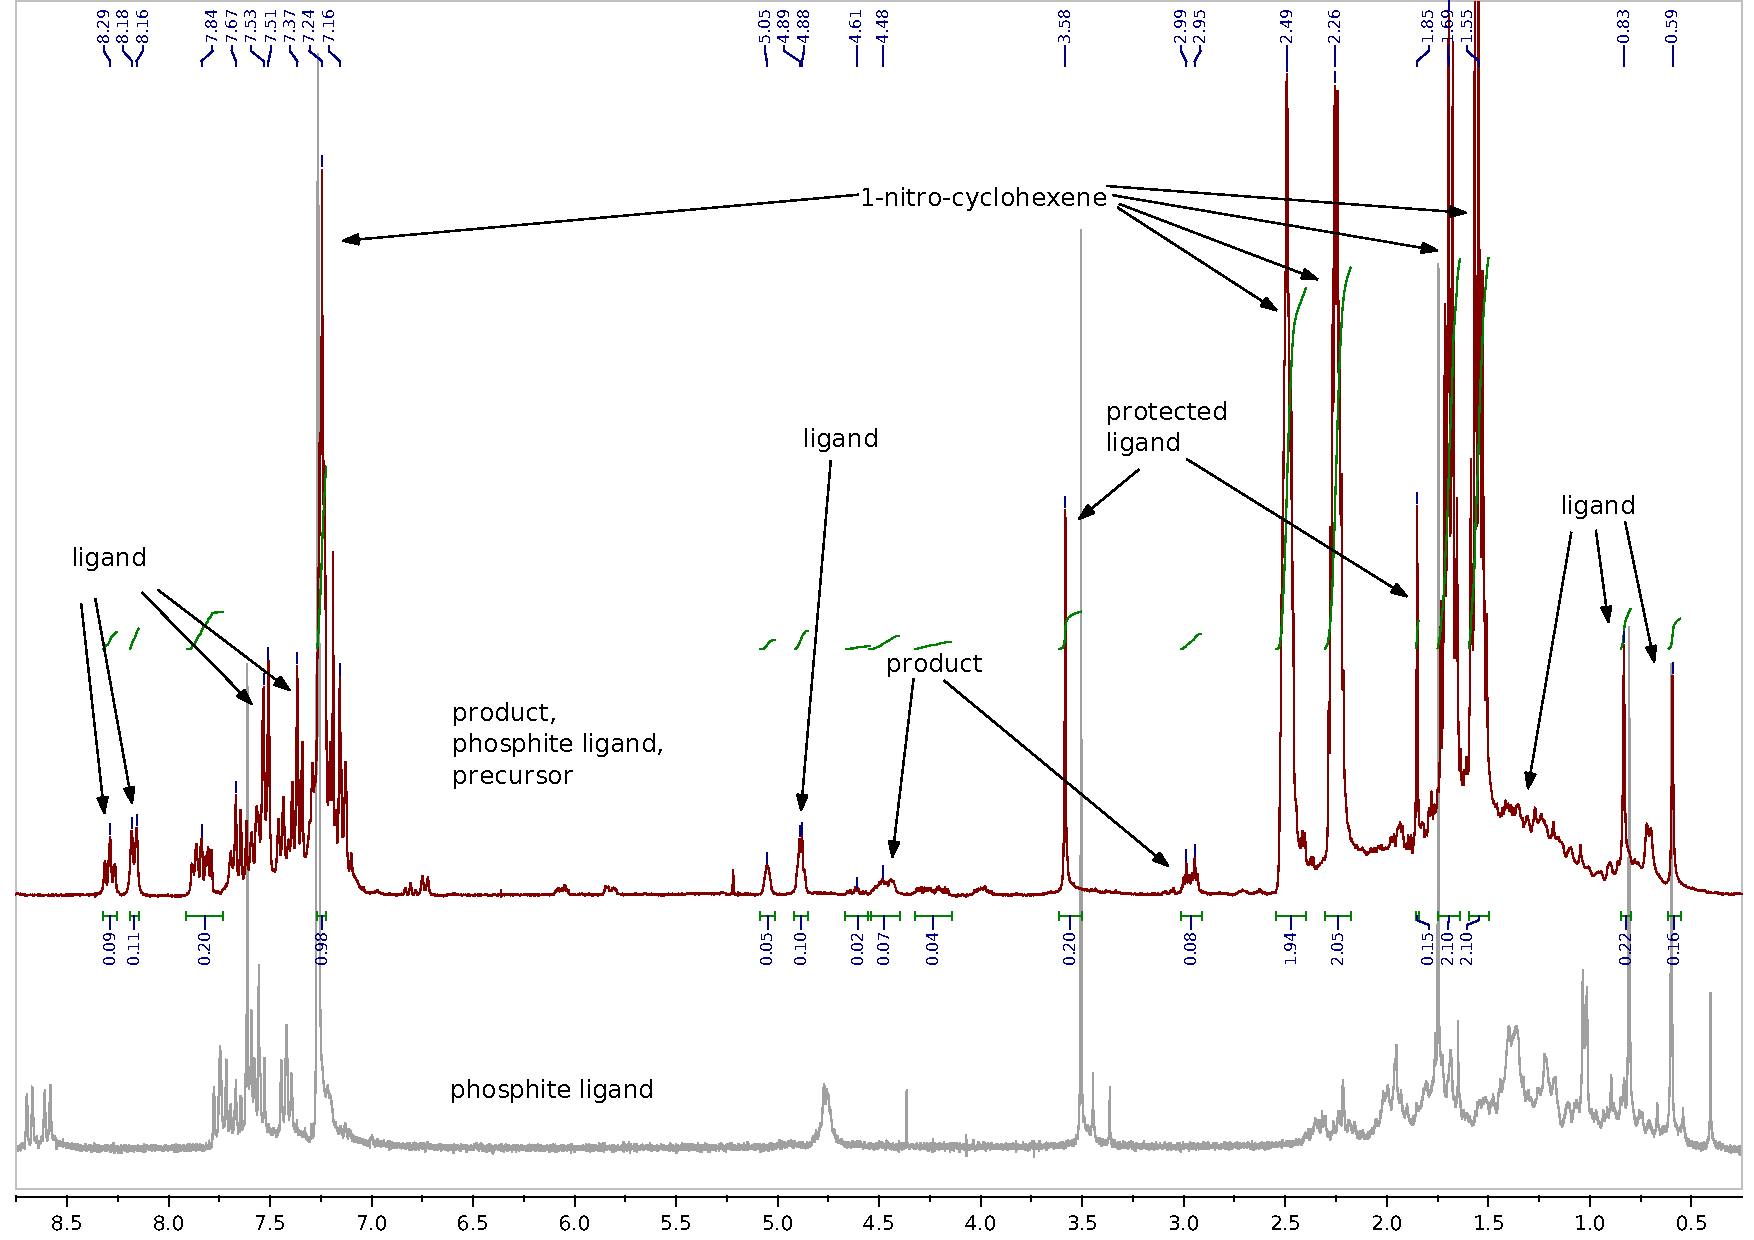
\includegraphics[width=1.4\textwidth]{sp/prodotto.pdf}
  \caption{Upper part: $^1$H-NMR (300~MHz, \ce{CDCl3}) spectrum of not pure (2-nitro-cyclo\-hexyl)benzene \cmpd+{ncb}. Identified impurities: ligand \cmpd+{legante}, deprotected ligand, 1-nitro\-cyclo\-hexene \cmpd{nc}. Lower part: $^1$H-NMR spectrum of the phosphite ligand \cmpd+{legante}.\label{sp:prodotto}}
\end{figure}
\else
\fignoeps
\fi
\end{landscape}
